\section{Gradient Methods - Part II}

\begin{definition}[]
	$\operatorname{prox}_\mathcal{C}(x)=$
	$\operatorname{argmin}_{y\in\mathcal{C}}\frac{1}{2}|x-y|^2$
	with $\mathcal{C}\subset \mathbb{R}^{n}$
\end{definition}

\begin{lemma}
	cl, cv
	$\mathcal{C}\subset \mathbb{R}^{n}$
	$\rightarrow$
	$|\operatorname{prox}_\mathcal{C}(x)-\operatorname{prox}_\mathcal{C}(y)|$
	$\le$
	$|x-y|$
	$\leftarrow$
	$|\operatorname{prox}_\mathcal{C}(x)-\operatorname{prox}_\mathcal{C}(y)|^2$
	$\le$
	$(\operatorname{prox}_\mathcal{C}(x)-\operatorname{prox}_\mathcal{C}(y))\T(x-y)$
\end{lemma}


\subsection{Projected Gradient Descent}

$x_{k+1}=\operatorname{prox}_\mathcal{C}(x_k-T\nabla f(x_k))$,
for $x_0,k_{0..N},T\in(0,2/L)$

\begin{proposition}
	$f$: $L$-sm, $\mu$-scv
	$\rightarrow$
	projected GD with
	$T=\frac{2}{L+\mu}$
	satisfies
	$|x_N - x^\star|\le$
	$|x_0 - x^\star|(1-\frac{2}{\kappa+1})^N$
	$(\kappa$ still $\frac{L}{\mu})$
\end{proposition}

\begin{lemma}
	$f:\mathbb{R}^{n}\rightarrow\mathbb{R}$, $L$-sm, \textbf{cv}
	$\rightarrow$
	$\tilde{f}$
	strongly-cv
	$\hat{f}(x) = f(x)+\frac{\mu}{2}|x-x_0|^2$
	and
	$|\tilde{x}^\star-x_0|\le|x^\star-x_0|$

	and
	$f(x)-f(x^\star)\le$
	$\tilde{f}(x)-\tilde{f}(\tilde{x}^\star)+$
	$\frac{\mu}{2}|x^\star-x_0|^2$,
	$\mu>0$
\end{lemma}

$\rightarrow$ from here one can apply GD or Nesterov, which results in:
$f(x_N)-f(x_0)\le\epsilon$
after
$N\sim L|x^\star-x_0|^2/\epsilon$
iterations

\begin{proposition}[Subgradient Method]
	cl, cv $\mathcal{C}$
	contained in ball of radius $R$,
	$x_{0..N-1}$ satisfy
	$f(\frac{1}{N}\sum_{k=0}^{N-1})-f(x^\star)$
	$\le\frac{RL_f}{\sqrt{N}}$
	under
	$x_{k+1} = \operatorname{prox}_\mathcal{C}(x_k-Tg_k)$
	$g_k\in\partial f(x_k)$,
	$T = \frac{R}{L_f\sqrt{N}}$
\end{proposition}


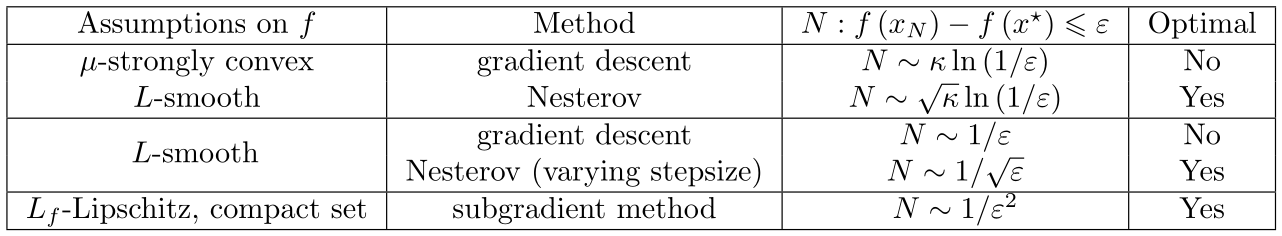
\includegraphics[width=\columnwidth]{images/table-gd-methods.png}

